\documentclass[a4paper]{article}
\usepackage{times}
\usepackage[utf8]{inputenc}
\usepackage{selinput}
\usepackage{upquote}
\usepackage[margin=2cm, rmargin=4cm, tmargin=3cm]{geometry}
\usepackage{tcolorbox}
\usepackage{xspace}
\usepackage[french]{babel}
\usepackage{url}
\usepackage{hyperref}
\usepackage{fontawesome5}
\usepackage{marginnote}
\usepackage{ulem}
\usepackage{tcolorbox}
\usepackage{graphicx}
%\usepackage[top=Bcm, bottom=Hcm, outer=Ccm, inner=Acm, heightrounded, marginparwidth=Ecm, marginparsep=Dcm]{geometry}


\newtcolorbox{Example}[1]{colback=white,left=20pt,colframe=slideblue,fonttitle=\bfseries,title=#1}
\newtcolorbox{Solutions}[1]{colback=white,left=20pt,colframe=green,fonttitle=\bfseries,title=#1}
\newtcolorbox{Conseils}[1]{colback=white,left=20pt,colframe=slideblue,fonttitle=\bfseries,title=#1}
\newtcolorbox{Warning}[1]{colback=white,left=20pt,colframe=warning,fonttitle=\bfseries,title=#1}

\setlength\parindent{0pt}

  %Exercice environment
  \newcounter{exercice}
  \newenvironment{Exercice}[1][]
  {
  \par
  \stepcounter{exercice}\textbf{Question \arabic{exercice}:} (\faClock \enskip \textit{#1})
  }
  {\bigskip}
  

% Title
\newcommand{\titre}{\begin{center}
  \section*{Algorithmes et Pensée Computationnelle}
\end{center}}
\newcommand{\cours}[1]
{\begin{center} 
  \textit{#1}\\
\end{center}
  }


\newcommand{\exemple}[1]{\newline~\textbf{Exemple :} #1}
%\newcommand{\attention}[1]{\newline\faExclamationTriangle~\textbf{Attention :} #1}

% Documentation url (escape \# in the TP document)
\newcommand{\documentation}[1]{\faBookOpen~Documentation : \href{#1}{#1}}

% Clef API
\newcommand{\apikey}[1]{\faKey~Clé API : \lstinline{#1}}
\newcommand{\apiendpoint}[1]{\faGlobe~Url de base de l'API \href{#1}{#1}}

%Listing Python style
\usepackage{color}
\definecolor{slideblue}{RGB}{33,131,189}
\definecolor{green}{RGB}{0,190,100}
\definecolor{blue}{RGB}{121,142,213}
\definecolor{grey}{RGB}{120,120,120}
\definecolor{warning}{RGB}{235,186,1}

\usepackage{listings}
\lstdefinelanguage{texte}{
    keywordstyle=\color{black},
    numbers=none,
    frame=none,
    literate=
           {é}{{\'e}}1
           {è}{{\`e}}1
           {ê}{{\^e}}1
           {à}{{\`a}}1
           {â}{{\^a}}1
           {ù}{{\`u}}1
           {ü}{{\"u}}1
           {î}{{\^i}}1
           {ï}{{\"i}}1
           {ë}{{\"e}}1
           {Ç}{{\,C}}1
           {ç}{{\,c}}1,
    columns=fullflexible,keepspaces,
	breaklines=true,
	breakatwhitespace=true,
}
\lstset{
    language=Python,
	basicstyle=\bfseries\footnotesize,
	breaklines=true,
	breakatwhitespace=true,
	commentstyle=\color{grey},
	stringstyle=\color{slideblue},
  keywordstyle=\color{slideblue},
	morekeywords={with, as, True, False, Float, join, None, main, argparse, self, sort, __eq__, __add__, __ne__, __radd__, __del__, __ge__, __gt__, split, os, endswith, is_file, scandir, @classmethod},
	deletekeywords={id},
	showspaces=false,
	showstringspaces=false,
	columns=fullflexible,keepspaces,
	literate=
           {é}{{\'e}}1
           {è}{{\`e}}1
           {ê}{{\^e}}1
           {à}{{\`a}}1
           {â}{{\^a}}1
           {ù}{{\`u}}1
           {ü}{{\"u}}1
           {î}{{\^i}}1
           {ï}{{\"i}}1
           {ë}{{\"e}}1
           {Ç}{{\,C}}1
           {ç}{{\,c}}1,
    numbers=left,
}

\newtcbox{\mybox}{nobeforeafter,colframe=white,colback=slideblue,boxrule=0.5pt,arc=1.5pt, boxsep=0pt,left=2pt,right=2pt,top=2pt,bottom=2pt,tcbox raise base}
\newcommand{\projet}{\mybox{\textcolor{white}{\small projet}}\xspace}
\newcommand{\optionnel}{\mybox{\textcolor{white}{\small Optionnel}}\xspace}
\newcommand{\advanced}{\mybox{\textcolor{white}{\small Pour aller plus loin}}\xspace}
\newcommand{\auto}{\mybox{\textcolor{white}{\small Auto-évaluation}}\xspace}


\usepackage{environ}
\newif\ifShowSolution
\NewEnviron{solution}{
  \ifShowSolution
	\begin{Solutions}{\faTerminal \enskip Solution}
		\BODY
	\end{Solutions}
  \fi}


  \usepackage{environ}
  \newif\ifShowConseil
  \NewEnviron{conseil}{
    \ifShowConseil
    \begin{Conseils}{\faLightbulb \quad Conseil}
      \BODY
    \end{Conseils}

    \fi}

    \usepackage{environ}
  \newif\ifShowWarning
  \NewEnviron{attention}{
    \ifShowWarning
    \begin{Warning}{\faExclamationTriangle \quad Attention}
      \BODY
    \end{Warning}

    \fi}
  

%\newcommand{\Conseil}[1]{\ifShowIndice\ \newline\faLightbulb[regular]~#1\fi}



\begin{document}

% Change the following values to true to show the solutions or/and the hints
\ShowSolutiontrue
\ShowConseiltrue
\titre
\cours{Prise en main de l'environnement de travail}

Le but de cette séance est d'installer et de configurer les outils qui seront utilisés tout au long du semestre. 

\subsection*{Prérequis}
Avant d'installer les outils de développement, vous devez vous assurer d'avoir installé Python et le kit de développement Java (Java).
\begin{enumerate}
    \item \textbf{Python}. Pour installer Python, rendez-vous sur le site officiel de Python \url{https://www.python.org/downloads}. Selectionnez la dernière version de Python et cliquez sur \textbf{Download}. Dans la page suivante, cliquez sur le fichier correspondant à votre système d'exploitation. \lstinline{macOS 64-bit installer} pour Mac et \lstinline{Windows x86-64 executable installer} pour Windows (processeurs 64 bits). Installez le fichier téléchargé. Pour tester que tout fonctionne, ouvrez votre terminal et tapez la commande \lstinline{python}, vous devriez avoir la fenêtre ci-dessous.
    
    \begin{figure}[h]
        \centering
        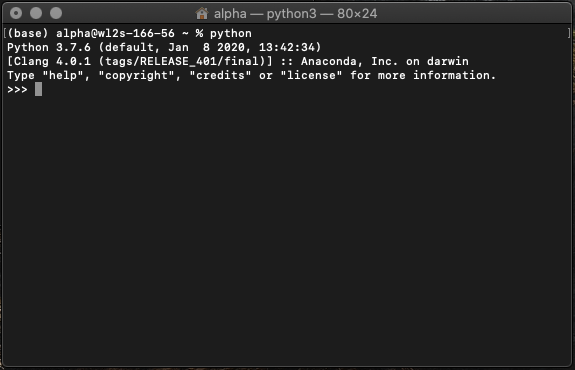
\includegraphics[width=1\textwidth]{img/python.png}
        \caption{Aperçu du terminal}
    \end{figure}

    \item \textbf{Java Development Kit (JDK)}. Le JDK contient tout le nécessaire pour développer des applications Java. Pour le télécharger, se rendre sur le site d'Oracle \url{https://www.oracle.com/java/technologies/downloads/} et sélectionner la version correspondant à votre système d'exploitation. Lire et accepter les conditions d'utilisation, cliquer sur \textit{Télécharger} et créer/se connecter à un compte Oracle pour procéder au téléchargement. Une fois le téléchargement terminé, installer le fichier.
\end{enumerate}

\begin{comment}

\subsection*{Pycharm}

Dans la première partie du cours, la plupart des notions présentées seront implémentées en Python. Dans ce tutoriel, nous vous indiquons comment utiliser un environnement de développement intégré (IDE) vous permettant d'écrire du code Python et de l'exécuter.\\
L'IDE qui sera utilisé tout au long du semestre sera Pycharm. Pour l'installer, suivez les étapes suivantes:
\begin{itemize}
    \item Cliquer sur le lien suivant pour télécharger le logiciel.
    \item Cliquer sur l'onglet correspondant à votre système d'exploitation et choisir la version \textbf{Professional}.
    \item Installer le logiciel et l'ouvrir.
    \item Remplir le formulaire suivant pour bénéficier d'une licence \url{https://www.jetbrains.com/shop/eform/students}.
    \item Une fois le formulaire envoyé, vous recevrez un email de confirmation. Suivre le lien pour obtenir une licence.
    \item Créer un compte JetBrains que vous utiliserez dans \textbf{Pycharm} pour utiliser votre IDE.

    \begin{figure}[h]
        \centering
        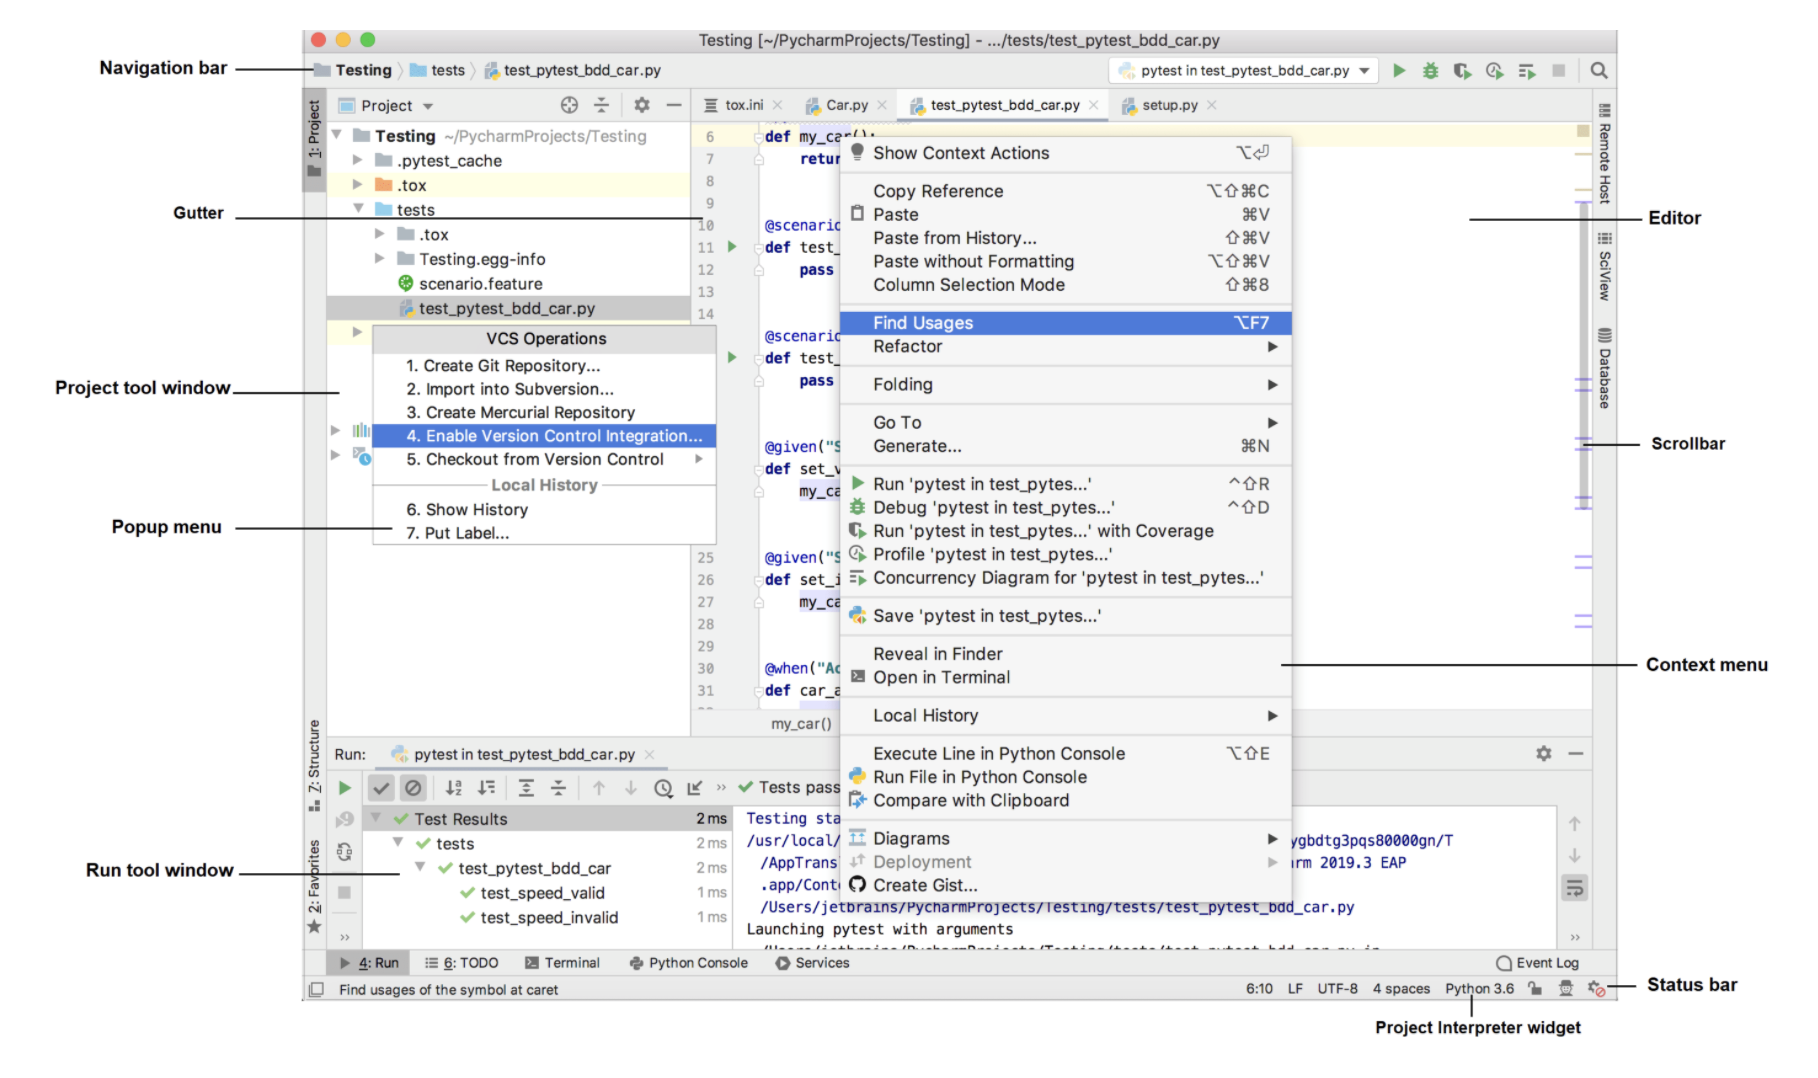
\includegraphics[width=1\textwidth]{img/pycharmUI.png}
        \caption{Interface utilisateur de Pycharm (\url{https://www.jetbrains.com/help/pycharm/guided-tour-around-the-user-interface.html}).}
    \end{figure}
\end{itemize}

\subsection*{Netbeans}
Dans la seconde partie du cours, les notions de programmation orientée objet seront principalement abordées en utilisant Java. L'un des IDE les plus utilisés pour programmer en Java est Netbeans. Pour ce cours, nous utiliserons une version récente de Netbeans ($>$ 8.0). Suivez les étapes suivantes pour l'installer:
\begin{itemize}
    \item Cliquer sur le lien suivant pour accéder à la page de téléchargement de Netbeans: \url{https://netbeans.apache.org/download/nb120/nb120.html}.
    \item Sélectionner le fichier correspondant à votre système d'exploitation, ensuite sélectionner le lien sous la rubrique \textbf{HTTP} et installer le fichier.
    \item Ouvrir Netbeans pour créer votre premier programme. Le lien suivant vous guidera vers la création d'un programme simple en Java: \url{https://netbeans.org/kb/docs/java/quickstart.html}.
\end{itemize}

\subsection*{Résolution Bug Windows}

Dans les exercices suivants, vous serez amenés à utiliser le shell de votre ordinateur. Il se peut que chez certaines personnes, certaines commandes recoivent ce message d'erreur lorsqu'elles sont executées : "Nom_de_la_commande n'est pas reconnue comme un commande interne ou externe." \\

Si vous obtenez ce message d'erreur, cela signifie que votre shell n'arrive pas à localiser le fichier de l'application que vous essayez d'utiliser (jdk (java) par exemple). Il va donc falloir aller ajouter le chemin vers cette application dans les varibales d'envrionnement. \\

Dans cette situation, assurez vous tout d'abord d'avoir bel et bien installé ladite application. Pour ce faire, allez dans votre explorateur de fichier, sur votre disque, sur "Programmes Files" puis cherchez l'application en question (ici java). Allez ensuite sur java et cherchez votre exécutable. Le chemin devrait ressembler à ça : "C:\Program Files\Java\jdk-14.0.2\bin". Si vous trouvez java dans le dossier bin, il est alors installé. Copiez alors votre chemin d'accès au dossier bin ("C:\Program Files\Java\jdk-14.0.2\bin" dans notre cas). \\

Pour finir, accédez aux variables d'environement : \\

tappez variables dans la barre de recherche, prenez "Modifier les variables d'environnement système". Cliquez sur "variables d'environnement" \\

Si vous avez déjà une variable nomée "Path" ou "PATH", modifiez la en ajoutant un ";" et en collant le chemin jusqu'au dossier ou votre application est stockée. Ici on ajoute donc ";C:\Program Files\Java\jdk-14.0.2\bin" \\

Deuxième cas, vous n'avez pas de variable "PATH" ou "Path". Créez en une, nommez la "Path" ou "PATH" et collez-y "C:\WINDOWS;C:\WINDOWS\system32". Collez ensuite ";" et le chemin jusqu'au dossier ou votre application est stockée. Ici on ajoute donc ";C:\Program Files\Java\jdk-14.0.2\bin" \\

Faites le pour "variables utilisateur", puis répétez l'opération pour "variables système" \\

Cliquez sur ok jusqu'à ce que toutes les fenêtres soient fermées, puis relancez votre shell. Le problème est normalement réglé. \\

N'hésitez pas à demander de l'aide aux assistants si vous n'y arrivez pas. \\

\begin{comment}
    % This section should be done in case we receive a confirmation that the exercise sessions will be done in the lab.

\subsection*{Utilisation des ordinateurs du Lab}
\end{comment}

\subsection*{IntelliJ}

L'IDE (Integrated Development Environment) qui sera utilisé tout au long du semestre sera \textbf{IntelliJ} dans son édition ultimate. Pour l'utiliser, vous devez suivre les étapes suivantes:
\begin{enumerate}
    \item Télécharger la version ultimate d'IntelliJ directement sur le site internet \url{https://www.jetbrains.com/idea/download/}, ensuite faites une demande pour obtenir une licence étudiante vous permettant d'activer la version ultimate d'IntelliJ. Vous pouvez le faire en suivant le guide suivant: \url{https://www.jetbrains.com/student/}.
    \item Pour utiliser Python sur IntelliJ, vous devez installer le plugin Python en cliquant ``Configure'' puis ``Plugins'' sur la fenêtre d'accueil d'IntelliJ. Cliquez sur ``Browse repositories'' pour chercher de nouveaux plugins.
    \item Pour créer un nouveau projet (Python par exemple), cliquez sur ``+ Create New Project'' à partir de la fenêtre d'accueil, sélectionnez Python sur le menu latéral. Définissez l'emplacement de votre SDK et donnez un nom à votre projet (Assurez-vous de choisir une version Python >= 3.5). Cliquez sur Ok.
\end{enumerate}

\subsection*{Résolution Bug Windows}

Sur Windows, lorsque vous tentez de run un fichier java, il se peut que le message d'erreur suivant s'affiche :\\

\begin{Example}{\faExclamationTriangle \quad Message d'erreur}
    \textbf{`javac' n'est pas reconnue comme une commande interne ou externe.}
\end{Example}

Dans ce cas, suivez les étapes suivantes :

\begin{enumerate}
    \item Ouvrez votre panneau de configuration $>$ Système et sécurité $>$ Système $>$ Paramètres systèmes avancés. La fenêtre suivante devrait s'afficher.\\
    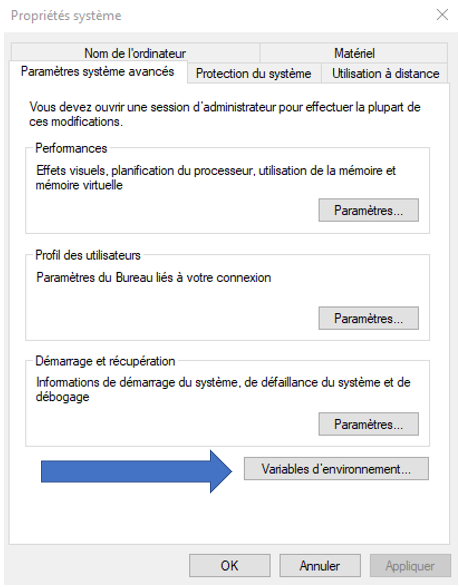
\includegraphics[height = 10cm]{img/Res1.PNG}
    \\
    \item Sélectionnez Variables d'environnement. Dans variables système, identifiez la variable "Path", sélectionnez là et choisissez modifier.\\
    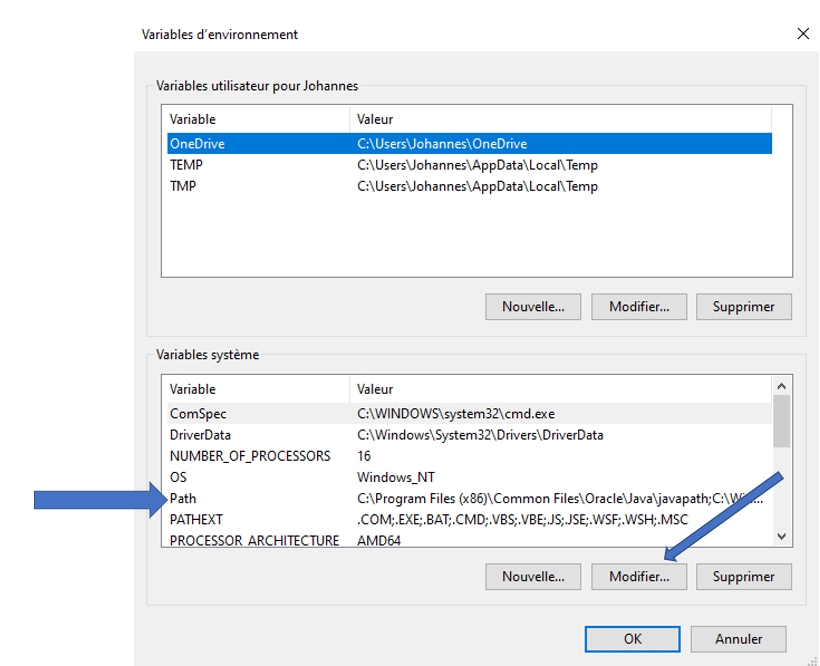
\includegraphics[width=16cm]{img/Res2.PNG}
    \item Ouvrez votre explorateur de fichiers et trouvez le chemin d'accès à \textbf{jdk\$\{votre version\} $>$ bin}. \\Par exemple : $C:\backslash Program Files\backslash Java\backslash jdk1.8.0\_261\backslash bin.$\\
    \item Copiez ce chemin d'accès et copiez-le à la dernière ligne de la variable d'environnement Path.\\\
    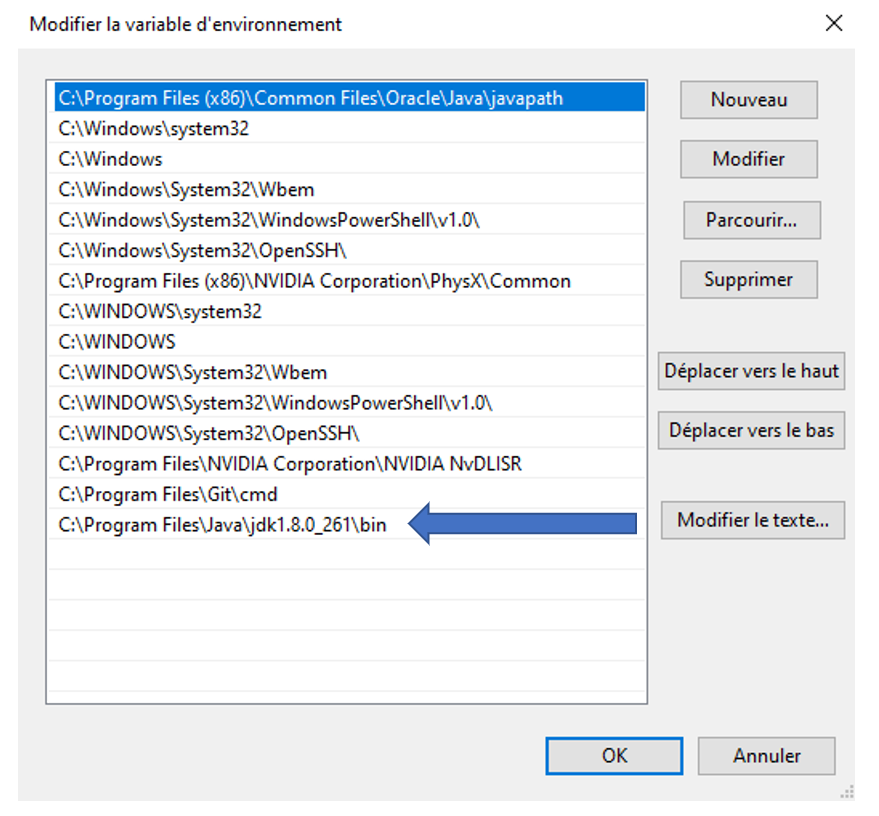
\includegraphics[width=15cm]{img/Res3.PNG}\\
    \item Faites ok. Puis redémarrez votre ordinateur.
    \item Ouvrez votre Terminal, Naviguez vers votre fichier .java et tapez :
        \begin{enumerate}
            \item \lstinline{javac VotreProgramme.java} (Cette commande va créer des fichiers.class)
            \item \lstinline{java VotreProgramme} (Cette commande va exécuter votre programme. A noter qu'il faut que votre programme doit être le fichier qui contient la classe \lstinline{main})
        \end{enumerate}
    
\end{enumerate}


\subsection*{Votre premier programme}

\begin{itemize}
    \item \textbf{Python: }\url{https://www.jetbrains.com/help/idea/creating-empty-python-project.html}
    \item \textbf{Java: }\url{https://www.jetbrains.com/help/idea/creating-and-running-your-first-java-application.html#run_app}
\end{itemize}

\end{document}
